%!TEX root=../master_thesis.tex

\chapter{Random Slicing}
\label{ch:random_slicing}
In this chapter we introduce the concept of \ac{RS} in detail.
The first section looks at \ac{RS} purely as a partitioning algorithm without considering replication.
Following this we discuss some simple approaches to integrate replication with \ac{RS}.

\section{Partitioning Algorithm}
\label{sec:partitioning_algorithm}
Miranda et al. have proposed \ac{RS}\cite{Miranda2014} as an ``efficient and scalable data placement for large-scale storage systems''.
The motivation to develop yet another data placement algorithm were several shortcomings of existing approaches like Consistent Hashing, especially when the cluster configuration changes often or scales to a high number of nodes.
The goal for the system is to keep a good adaptivity and fairness when scaling a cluster while keeping look-up time and memory consumption low and supporting redundancy in the cluster.
\emph{Adaptivity} here means the ability to reconfigure the cluster without moving unnecessary data points stored on it.
\emph{Fairness} is defined as the ability to distribute data and requests to nodes according to their capacity.

The basic principle of \ac{RS} is to assign one or more sections on the unit interval $[0,1)$ to each node in the cluster such that
\begin{enumerate}
	\item no assigned sections overlap,
	\item the interval is assigned completely,
	\item the sum of length of all sections assigned to a given node is equal to its relative capacity with respect to the total cluster capacity.
\end{enumerate}
This basic functionality can be seen as another variant of Consistent Hashing\cite{Fritchie2018}.

In detail the system starts with an initial configuration of nodes $n_1,...,n_k$ with capacities $c_1,...,c_k$ and relative capacities
\[
	r_i = \frac{c_i}{\sum\limits_{j=1}^kc_j}.
\]
The unit interval is simply split into intervals of length $r_i$ and each node is assigned the respective section.
Whenever the cluster configuration changes, either by removing nodes, adding nodes or by changing the capacity of existing nodes, new relative capacities for all nodes are computed.
Using the current assignment map and the new relative capacities a \emph{gap collection} algorithm chooses which sections of the current mapping are split or completely reassigned.
The authors propose and examine two simple algorithms and a sorted variant for each.
They determine that the \emph{CutShift+Sorted} algorithm yields the best results with respect to keeping the number of new sections low, which is the biggest influence on memory consumption and lookup time.
This algorithm tries to release only complete intervals first and alternates between splitting at the start and at the end of sections if splits are necessary to get bigger gaps.
The sorted variant in addition assigns the nodes with the highest capacity to the largest gaps.

However, Scott Fritchie, the Riak developer who proposed using \ac{RS} with Riak Core\cite{Fritchie2018}, implemented a greedy algorithm\footnote{\url{https://github.com/basho/machi/blob/master/src/machi_chash.erl}} for a different project which minimizes data transferred between nodes when the cluster is changed, as data transfers over a distributed network can be a bottle neck\cite{Fritchie2018}.
Its pseudocode can be found in Algorithm \ref{alg:gap_collection}.
This algorithm starts with computing the signed difference of relative capacities (\cref{line:gap_collection_diffs1,line:gap_collection_diffs2,line:gap_collection_diffs3}).
Then, for each node with shrinking relative capacities gaps are collected greedily by iterating their sections and marking sections as unused until they meet the capacity difference (\cref{line:gap_collection_neg1,line:gap_collection_neg2,line:gap_collection_neg3,line:gap_collection_neg4,line:gap_collection_neg5,line:gap_collection_neg6,line:gap_collection_neg7,line:gap_collection_neg8,line:gap_collection_neg9,line:gap_collection_neg10,line:gap_collection_neg11,line:gap_collection_neg12,line:gap_collection_neg13}).
At most one section is split per node, which happens if the currently viewed section is larger than the remaining difference.
The created gaps are then greedily assigned to the nodes with a growing relative capacity in the same manner (\cref{line:gap_collection_pos1,line:gap_collection_pos2,line:gap_collection_pos3,line:gap_collection_pos4,line:gap_collection_pos5,line:gap_collection_pos6,line:gap_collection_pos7,line:gap_collection_pos8,line:gap_collection_pos9,line:gap_collection_pos10,line:gap_collection_pos11,line:gap_collection_pos12,line:gap_collection_pos13,line:gap_collection_pos14,line:gap_collection_pos15}).
Therefore, at most one gap is split per node for the same reasons.
Now that the complete interval is assigned, neighboring sections with the same owner are merged into one section (\cref{line:gap_collection_merge}).

\begin{algorithm}
\caption{Gap Collection}
\label{alg:gap_collection}
\SetKwData{Sections}{sections}
\SetKwData{Capacities}{capacities}
\SetKwData{OldCapacities}{old\_capacities}
\SetKwData{CapacityDiff}{capacity\_diff}
\SetKwData{RelCapacities}{rel\_capacities}
\SetKwData{Unowned}{unowned}
\SetKwFunction{GetOwner}{GetOwner}
\SetKwFunction{SetOwner}{SetOwner}
\SetKwFunction{Length}{Length}
\SetKwFunction{Split}{Split}
\SetKwFunction{Append}{Append}
\SetKwFunction{Replace}{Replace}
\SetKwFunction{NextUnowned}{NextUnowned}
\SetKwFunction{MergeSameNeighbors}{MergeSameNeighbors}
\KwData{List of sections \Sections, List of new relative capacities \Capacities}
\KwResult{New assignment of sections to nodes \Sections}
\For{$s\in\Sections$}{
 $\OldCapacities[\GetOwner{s}] \leftarrow \OldCapacities[\GetOwner{s}] + \Length{s}$
}
\For{$\{o, c\}\in\Capacities$}{\label{line:gap_collection_diffs1}
 $\CapacityDiff[o]\leftarrow c - \OldCapacities[o]$\;\label{line:gap_collection_diffs2}
}\label{line:gap_collection_diffs3}
\For{$s\in\Sections$}{
 $o \leftarrow \GetOwner{s}$\;
 $d \leftarrow \CapacityDiff[o]$\;
 $l\leftarrow \Length{s}$\;
 \If{$d < 0$}{\label{line:gap_collection_neg1}
  \If{$|d|\leq l$}{\label{line:gap_collection_neg2}
   $\{s_1,s_2\}\leftarrow \Split{s, l - |d|}$\;\label{line:gap_collection_neg3}
   $s_2\leftarrow\SetOwner{$s_2$, \Unowned}$\;\label{line:gap_collection_neg4}
   $\Sections\leftarrow\Replace{\Sections, s, ($s_1$, $s_2$)}$\;\label{line:gap_collection_neg5}
   $\CapacityDiff[o]\leftarrow 0$\;\label{line:gap_collection_neg6}
  }\label{line:gap_collection_neg7}
  \If{$|d| > l$}{\label{line:gap_collection_neg8}
   $s\leftarrow\SetOwner{s, \Unowned}$\;\label{line:gap_collection_neg9}
   $\Sections\leftarrow\Replace{\Sections, s, s}$\;\label{line:gap_collection_neg10}
   $\CapacityDiff[o]\leftarrow d + l$\;\label{line:gap_collection_neg11}
  }\label{line:gap_collection_neg12}
 }\label{line:gap_collection_neg13}
}
\For{$(o,d)\in\CapacityDiff$}{
 \While{$d > 0$}{\label{line:gap_collection_pos1}
  $s \leftarrow \NextUnowned{\Sections}$\;\label{line:gap_collection_pos2}
  $l\leftarrow \Length{s}$\;\label{line:gap_collection_pos3}
  \If{$|d|\leq l$}{\label{line:gap_collection_pos4}
   $\{s_1,s_2\}\leftarrow \Split{s, l - |d|}$\;\label{line:gap_collection_pos5}
   $s_1\leftarrow\SetOwner{$s_1$, o}$\;\label{line:gap_collection_pos6}
   $\Sections\leftarrow\Replace{\Sections, s, ($s_1$, $s_2$)}$\;\label{line:gap_collection_pos7}
   $\CapacityDiff[o]\leftarrow 0$\;\label{line:gap_collection_pos8}
  }\label{line:gap_collection_pos9}
  \If{$|d| > l$}{\label{line:gap_collection_pos10}
   $s\leftarrow\SetOwner{s, o}$\;\label{line:gap_collection_pos11}
   $\Sections\leftarrow\Replace{\Sections, s, s}$\;\label{line:gap_collection_pos12}
   $\CapacityDiff[o]\leftarrow d - l$\;\label{line:gap_collection_pos13}
  }\label{line:gap_collection_pos14}
 }\label{line:gap_collection_pos15}
}
$\Sections \leftarrow \MergeSameNeighbors{\Sections}$\;\label{line:gap_collection_merge}
\Return \Sections\;
\end{algorithm}

Determining the node a given key belongs to can be achieved by applying a hash function to the key and mapping the hash space to the unit interval.
This is done both for storing and retrieving data.
Redundancy can be achieved by different strategies and only some simple solutions are given in the original paper.
We discuss some simple approaches to solving the redundancy problem in Section \ref{sec:replication_placement_strategy}.

In addition to the description of their approach, Miranda et al.\cite{Miranda2014} conducted an analysis on different data placement strategies including two variants of Consistent Hashing in a simulated environment to compare them with respect to fairness, memory usage, lookup time, and adaptivity.
The summary of their qualitative results can be found in Table \ref{tab:random_slicing_analysis} taken from the original paper\cite{Miranda2014}.
As one can see \ac{RS} performs better than the other strategies when looking at each of their weak points.
It is however important to note that the analysis was done for large-scale system together with high redundancy for which some of the strategies were not developed.
As mentioned before the adaptivity can be improved by using a different gap collection algorithm at the cost of memory usage and lookup time.

Figure \ref{fig:random_slicing_example} shows an example of \ac{RS} with Fritchie's gap collection algorithm .
In this example the unit interval is interpreted as a ring running clockwise with the 0/1 point at the top like in Consistent Hashing to make a comparison easier.
The used nodes all have the same capacity.
In the example each ring represents a configuration of the cluster, with the most outward ring being the initial and the inner ring being the final configuration.
Initially 4 nodes get assigned a quarter of the ring each.
In the second configuration one node is added.
The new node takes an equal part of each existing section such that each node owns a fifth of the interval.
Two new nodes are added in the next step.
One can see, that some small intervals are reassigned completely and some are split.
The transition is from 7 to 10 nodes in which one can easily see the mechanism of splitting gaps while assigning nodes.
The fact that gaps are only assigned to new nodes implies that there are no transfers of data between existing nodes.
This shows that the amount of transferred data is optimal for each reconfiguration.

\begin{figure}
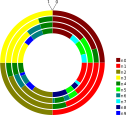
\includegraphics[width=\textwidth]{random_slicing_example}
\caption[Random Slicing example]{Random Slicing example scaling from 4 to 5 to 7 to 10 nodes with homogeneous capacity.}
\label{fig:random_slicing_example}
\end{figure}

\begin{table}
\begin{tabularx}{\textwidth}{|l|X|X|X|X|}
\hline
Strategy & Fairness & Memory usage & Lookup time & Adaptivity\\
\hline
\emph{Consistent Hashing (fixed)} & Poor & High & Moderate & Good\\
\emph{Consistent Hashing (adapt.)} & Moderate & High & High & Poor\\
\emph{Redundant Share} & Good & Low & Very High & Good\\
\emph{$\text{RUSH}_\text{P}$} & Poor & Low & Very High & Very Good\\
\emph{$\text{RUSH}_\text{R}$} & Good for low number of replicas & Low & Low &Very Good\\
\emph{$\text{RUSH}_\text{T}$} & Good & Low & Very High & Very Good\\
\emph{Random Slicing} & Good & Low & Low & Good\\\hline
\end{tabularx}
\caption[Qualitative analysis of different data placement strategies]{Qualitative analysis of different data placement strategies. Reprinted from \cite{Miranda2014}.}
\label{tab:random_slicing_analysis}
\end{table}

\section{Replication Placement Strategy}
\label{sec:replication_placement_strategy}
After the initial node to store a data block by its key is chosen through hashing on the intervals created by \ac{RS}, additional $N-1$ copies have to be distributed to $N-1$ distinct physical nodes.
For the correctness of \acp{RPS} it is assumed that the system configuration is correct, which means at times of operational states there are $n \geq N$ physical nodes in the cluster and $R \leq W \leq N$.
The \ac{RPS} should return a preference list of at least $N$ nodes, where the initial node is the head and the tail consists of nodes where replicas are stored in descending preference.

Load balancing between all nodes should be achieved at least asymptotically such that it gets closer to the ideal value when the ratio of replicas to nodes in the cluster $\frac{N}{n}$ gets smaller.
Considering only the primary replica, i.e. the head of the preference list, a placement strategy should always achieve perfect load balancing for a uniform distribution of data.
The ideal case is that for relative capacities $c_1,..,c_n$ of the nodes their relative load $l_i$ should be equal to the capacity $c_i$.
The relative capacity of node $n_i$ with weight $w_i$ is $c_i = \frac{w_i}{\sum_{j=1}^{n}w_j}$.
The relative load of node $n_i$ after $k$ keys have been distributed and $k_i$ keys are stored on $n_i$ is $l_i = \frac{k_i}{Nk}$.

To support the gossip protocol and local functionality of \ac{RCL} the replication strategy must not use a central server or other communication between the nodes.
The result should only be based on the current local view.
If two local views are the same, the preference list should be the same, i.e be deterministic.


\subsection{Random Replication}
This simple approach uses the outputs of a random uniform function as keys until $N$ distinct physical nodes are hit.
To achieve the same preference list for the same partitioning across all nodes the random function is seeded with the initial key.
A pseudo code  version of the algorithm is shown in Algorithm \ref{alg:trivial}.
Random Replication was chosen by Miranda et al. as the replication strategy in the analysis of \ac{RS}\cite{Miranda2014}.
Initially Brinkmann et al. mention this approach as a motivation for Redundant Share\cite{Brinkmann2007}.
Theoretical results showing non-optimal capacity usage in a heterogeneous system seem to have a neglectable impact on load balancing according to the simulations done by Miranda et al.

\begin{algorithm}
\caption{Trivial Replication}
\label{alg:trivial}
\SetKwData{Preflist}{preflist}
\SetKwData{Secs}{secs}
\SetKwFunction{GetNode}{GetNode}
\SetKwFunction{Length}{Length}
\SetKwFunction{Append}{Append}
\SetKwFunction{Rand}{Rand}
\KwData{List of sections \Secs, number of required replicas $N$, key of data to be replicated $k$}
\KwResult{\Preflist of at least length $N$}
$i \leftarrow 0$\;
$\Preflist \leftarrow \emptyset$\;
\While{\Length{\Preflist} $< N$}{
	$r \leftarrow \Rand{i, k}$\;
	\If{\GetNode{\Secs, $r$}$\notin$ \Preflist}{
				\Append{\Preflist, \GetNode{\Secs, $r$}}\;
	}
	$i \leftarrow i + 1$\;
}
\end{algorithm}

\subsubsection{Worst Case Runtime}
Since the process of finding nodes to store replicas on is random the worst case is that not enough nodes are hit after a finite number of steps and the replication algorithm does not terminate.
However, this is highly improbable.
We show this by computing probabilities of a fixed node with relative capacity $c$ being picked after $k$ steps.
To this end we model a random experiment with the geometric distribution.
Each independent trial has a probability of $c$ that the fixed node is drawn and $1-c$ that it is not drawn.
Therefore the probability to draw the node after exactly $k$ steps is
\[
	Pr(X=k)=(1-c)^{k-1}c,
\]
the expected value for $k$ is
\[
	E(X)=\frac{1}{c}
\]
and the probability to draw the node after at most $k$ steps is
\[
	Pr(X\leq k)=\sum\limits_{i=1}^{k}(1-c)^{i-1}c=c\sum\limits_{i=0}^{k-1}(1-c)^{i}=c\frac{(1-c)^0-(1-c)^{k}}{1-(1-c)}=1-(1-c)^k.
\]
Solving the inequality $Pr(X\leq k) = 1-(1-c)^k \geq p$ for $k$ yields
\[
	k \geq \log_{1-c}(1 - p)
\]
and therefore the minimal value fulfilling this inequality is
\[
	k=\lceil\log_{1-c}(1 - p)\rceil
\]

To further illustrate these values first we choose three different scenarios and compute $E(X)$, $Pr(X\leq k)$ for $k\in\{i\cdot n\mid i\in\{1,...,5\}\}$, and the minimal values for $k$ such that $Pr(X\leq k)\geq 0.95$ and $Pr(X\leq k)\geq 0.99$.
The first scenario $S_1$ is derived from the example shown in \cref{fig:random_slicing_example}.
Here there are 10 homogeneous nodes with the same capacity.
Therefore $n_1=10$ and $c_1=0.1$.
The second scenario $S_2$ is motivated by a high scaling with 1000 homogeneous nodes.
Therefore $n_2=1000$ and $c_2=0.001$.
The last scenario $S_3$ represents a heterogeneous system in which we consider a node with only a tenth of the average capacity.
We choose $n_3=10$ and $c_3=0.01$

The numbers for those scenarios are shown in \cref{tab:probabilities}.
An interesting aspect is that for the homogeneous scenarios all values appear to scale with the number of nodes.
The number of steps needed to guarantee that a given node is chosen with a specific probability also scales with the ratio of the actual capacity of the node to the average capacity.
While these results are not surprising when looking at the equation we intend to give an easier understanding with those examples.


\begin{table}
\begin{tabularx}{\textwidth}{|l|X|X|X|X|X|X|X|X|}
\hline
Scenario & $E(X)$ & $Pr_{1n}$ & $Pr_{2n}$ & $Pr_{3n}$ & $Pr_{4n}$ & $Pr_{5n}$ & $k_{0.95}$ & $k_{0.99}$\\\hline
$S_1$ & 10 & 0.651 & 0.878 & 0.958 & 0.985 & 0.995 & 29 & 44\\
$S_2$ & 1000 & 0.632 & 0.865 & 0.950 & 0.982 & 0.993 & 2994 & 4603\\
$S_3$ & 100 & 0.182 & 0.331 & 0.453 & 0.552 & 0.634 & 298 & 458\\
\hline
\end{tabularx}
\caption[Example Probabilities with Random Replication]{Example Probabilities with Random Replication. Shows expected value for $k$, probabilities that the node is chosen within a given number of steps and number of steps needed to be chosen with a given probability.}
\label{tab:probabilities}
\end{table}


\subsubsection{Example}
Using the final ring from the example in Figure \ref{fig:random_slicing_example} and the key $0.345$ the resulting preference list is \lstinline![n1,n8,n4,n9,n5,n2,n7,n6,n0,n3]!.
The random algorithm used to create the random keys is Erlang's implementation of the Xorshift116 generator combined with the StarStar scrambler\cite{Blackman2018}.

\subsubsection{Discussion}
Using random replication leads to near perfect load balancing according to simulations by Miranda et al\cite{Miranda2014}.
It is highly unlikely that the same node is drawn over and over when the ratio of available nodes to required nodes is high enough and therefore the runtime can be expected to be nearly linear in the number of required nodes.
Since the random function is seeded with the primary key, the placement on the unit interval of replica candidates is deterministic for each key.
Therefore after a cluster reconfiguration not all replica placements have to be recomputed as they can be moved to the node now responsible for that section.
Recomputation is only necessary if the positions of two replicas are owned by the same node after a reconfiguration and therefore the preference list not having enough distinct members.

\subsection{Ring Rotation}
Another approach has the intention of keeping Riak Core's ring structure and making use of it.
A pseudo code version of this algorithm is shown in  Algorithm \ref{alg:ring_rotation}.
The ring rotation is visualized in Figure \ref{fig:ring_rotation}.
Its idea is to stepwisely rotate the ring counter-clockwise, or from another perspective, the key clockwise, by the lengths of its sections and use the original hash value to create the preference list.
The aim of this approach is to achieve load balancing by considering the lengths of the sections.
However, there is a possibility that after a whole rotation of the ring less than $N$ nodes are in the preference list.
To overcome this, in the $i$-th rotation the sections are split into $2^i$ subsections and therefore the rotation step lengths get shorter (\cref{line:rotation_step}).
This leads to smaller segments that were previously skipped by rotating by a bigger length to be added to the preference list.
Since the rotation of the subsections leads to querying the same key value multiple times, a small optimization would be to skip those values (\cref{line:rotation_skip}).
This is done by rotating the ring by $\frac{1}{2^i}$ of the original length once to offset the value, then rotate it $2^{i-1}-1$ times by $\frac{1}{2^{i-1}}$  of the original length and finally the offset is reverted without querying the ring.
Implementation wise instead of the ring being rotated counter-clockwise the key is rotated around the ring clockwise.

\begin{algorithm}
\caption{Rotation for each segment}
\label{alg:ring_rotation}
\SetKwData{Preflist}{preflist}
\SetKwFunction{Length}{Length}
\SetKwFunction{GetNode}{GetNode}
\SetKwFunction{GetLength}{GetLength}
\SetKwFunction{Append}{Append}
\SetKwFunction{SubList}{SubList}
\KwData{Mapping of ranges to nodes $m$, number of required replicas $N$, index of data to be replicated $k$}
\KwResult{\Preflist of at least length $N$}
$i \leftarrow 0$\;
$\Preflist \leftarrow \emptyset$\;
$m \leftarrow \Append{\SubList{m, \GetNode{k}, \Length{m}}, \SubList{0, \GetNode{k}}}$\;
\While{\Length{\Preflist} $< N$}{
	\For{$s \in m$}{
		$step \leftarrow \GetLength{s}\cdot 2^{-i}$\;\label{line:rotation_step}
		\tcp{One step to offset the key}
		$k \leftarrow (k + step)$\;
		\If{$k \geq 1.0$}{
			$k \leftarrow k - 1.0$\;
		}
		\If{\GetNode{$m$, $k$}$\notin$ \Preflist}{
			\Append{\Preflist, \GetNode{$m$, $k$}}\;
		}
		\tcp{Skip previously visited indices}
		\For{$j \leftarrow 1$ \KwTo $2^{i-1}-1$}{
			
			$k \leftarrow (k + 2\cdot step)$\;\label{line:rotation_skip}
			\If{$k \geq 1.0$}{
				$k \leftarrow k - 1.0$\;
			}
			\If{\GetNode{$m$, $k$}$\notin$ \Preflist}{
				\Append{\Preflist, \GetNode{$m$, $k$}}\;
			}
		}
		\tcp{One step to change offset to first index of the next node without lookup}
		$k \leftarrow (k + step)$\;
		\If{$k \geq 1.0$}{
			$k \leftarrow k - 1.0$\;
		}
	}
	$i \leftarrow i + 1$\;
}
\Return{\Preflist}
\end{algorithm}

\begin{figure}
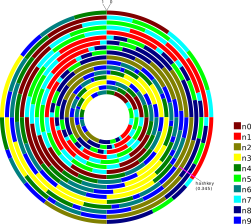
\includegraphics[width=\textwidth]{random_slicing_rotation}
\caption[Visualization of the ring rotation replication]{Visualization of the ring rotation replication.
n0...n9 are the physical nodes.
The ring is rotated counterclockwise by the length of each section.
From the outer to the inner ring each rotation step is shown.
}
\label{fig:ring_rotation}
\end{figure}

\subsubsection{Correctness}
The algorithm is seen as correct if it constructs a preference list of $N$ distinct physical nodes for any correct system configuration with $n\geq N$ nodes.
The maximum rotation length will be eventually smaller than the shortest section.
Therefore after a finite amount of rotations each section on the ring will be queried which leads to a preference list containing each physical node.
Since the system configuration is assumed to be correct the preference list contains at least $N$ distinct physical nodes.

\subsubsection{Worst Case Runtime}
In the worst case $N$ is equal to the number of distinct physical nodes and the ring actually has to rotate the maximum number of rounds.
 Let $s$ be number of segments, $l_{max}$ length of the largest segment, $l_{min}$ length of the shortest segment.
Starting with round $i=0$ the number of steps per round is $r(i) = 2^i\cdot s$
Therefore the total number of steps for $k$ rounds is
\[
\sum\limits_{i=0}^{k-1}2^i\cdot s = s\cdot \sum\limits_{i=0}^{k-1}2^i = s\cdot\frac{1-2^k}{1-2} = (2^k - 1)\cdot s
\]
and the number of rounds in the worst case is
\begin{align*}
\frac{l_{max}}{2^k} &\leq l_{min}\\
\frac{l_{max}}{l_{min}} &\leq 2^k\\
k &\geq \log_2(\frac{l_{max}}{l_{min}})\\
k &= \lceil \log_2(\frac{l_{max}}{l_{min}}) \rceil.
\end{align*}

\subsubsection{Load Balancing}
\ac{RS} guarantees load balancing for the primary copy of a data item.
Looking at Figure \ref{fig:ring_rotation} one can see that sections owned by the same node do overlap from one rotation step to another.
This complicates a quantitative analysis of load balancing and we have to rely on simulated data for quantitative results.
However, the overlaps intuitively lead to an imperfect load balancing as the overlapping section is unused in all rotation steps but the first it appears in.

\subsubsection{Example}
Using the example from Figure \ref{fig:ring_rotation} and hash key $0.345$, the resulting preference list is \lstinline![n1,  n8, n2, n9, n4, n3, n6, n0, n5, n7]!.
To achieve a preference list for $N=3$, 3 rotation steps are necessary for that key.
To achieve a preference list for $N=10$, 15 rotation steps are necessary for that key.

\subsubsection{Discussion}
From the initial look the ring rotation replication seems to be sub-optimal both with respect to the expected runtime as well as the expected load balancing.
Since the rotations are based on the length of sections a reconfiguration of the cluster leads to a total rearrangement of replica placements.
Overall this approach does not look like a promising solution to the placement of replicas.

\subsection{Ring Jumping}
Similar to the ring rotation approach ring jumping  makes use of the original ring structure.
A pseudo code version of the algorithm is shown in Algorithm \ref{alg:ring_jumping} and a visualization can be seen in Figure \ref{fig:ring_jumping}.
However, instead of rotating the ring in the order of its sections it is rotated by the length of the section the key currently belongs to.
This is repeated until $N$ distinct physical nodes are added to the preference list.

\begin{algorithm}[H]
\caption{Ring Jumping}
\label{alg:ring_jumping}
\SetKwData{Preflist}{preflist}
\SetKwData{Secs}{secs}
\SetKwFunction{GetLength}{GetLength}
\SetKwFunction{GetNode}{GetNode}
\SetKwFunction{Append}{Append}
\KwData{List of sections \Secs, number of required replicas $N$, index of data to be replicated $k$}
\KwResult{\Preflist of at least length $N$}
$\Preflist \leftarrow \emptyset$\;
\While{\Length{\Preflist} $< N$}{
	$k \leftarrow k + \GetLength{\Secs, k}$\;
	\If{$k \geq 1.0$}{
				$k \leftarrow k - 1.0$\;
	}
	\If{\GetNode{\Secs, $k$}$\notin$ \Preflist}{
				\Append{\Preflist, \GetNode{\Secs, $k$}}\;
	}
}
\end{algorithm}

\begin{figure}
\centering
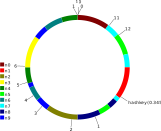
\includegraphics[width=0.5\textwidth]{random_slicing_jumping}
\caption{Ring Jumping}
\label{fig:ring_jumping}
\end{figure}

\subsubsection{Correctness}
Assume that the key is rotated around the ring such that it is within the initial section again for the first time.
If it is at its exact starting place then the sum of lengths of sections it hit is 1, which can only be the case if it visited every section and therefore every physical node was added to the preference list.
Otherwise, the starting place of the key for the next rotation is less than the initial one.
Then there is a chance that segments that where skipped before are now added to the preference list.
This is done until the key is at an initial position between the start of the starting section and its offset by the length of the shortest section.
Then it is guaranteed that every section is visited in the following rotation.

\subsubsection{Worst Case runtime}
The worst case occurs when the initial key is at the right edge of the longest segment and the shortest segment has to be visited.
Additionally only the shortest segment is not visited and therefore the position offset for each round is minimal.
Let $s$ be number of segments, $l_{max}$ length of the largest segment, $l_{min}$ length of the shortest segment.
Assume that only the shortest segment is not visited.
Therefore the start index of the next round moves by $l_{min}$: $s_{i+1} = s_{i} - l_{min}$.
The shortest segment is guaranteed to be hit in round $k$ if $s_k \leq l_{min}$.
So the number of rounds needed is $\lceil\frac{l_{max}}{l_{min}}\rceil$ and the number of steps needed is $s\cdot\lceil\frac{l_{max}}{l_{min}}\rceil$.

\subsubsection{Load Balancing}
Analyzing load balance properties of jumping approach qualitatively is complicated by the influence of section lengths and order.
Assuming equal section length and distribution this approach is equivalent to Riak Core's \ac{RPS} as the $N$ next sections are chosen by definition.
Abstracting from this special case the load on a section is expected to scale with its relative size.
However, the actual numbers need to be determined experimentally in a simulated environment.

\subsubsection{Example}
In Figure \ref{fig:ring_jumping} one can see how the $10$ nodes are selected for the preference list for the key $0.345$.
This results in \lstinline![n1, n8, n2, n9, n6, n3, n0, n7, n5]!.
Defining the \emph{efficiency} of the approach by the ratio of number of selected nodes to number of queries shows an efficiency of $100\%$ for the first six nodes.
To get a complete preference list with $10$ nodes 13 queries are required resulting in an efficiency of $76.9\%$.

\subsubsection{Discussion}
While not having the best expected runtime and unknown load balancing after the initial look this approach still has the potential to prove itself as a feasible solution for the replica placement in simulations.
As the approach is derived from Riak Core's algorithm it may also make visualizing differences easier.
One drawback of the approach is the dependency on the length and order of sections.
This creates a need to recompute the replica placements for any cluster reconfiguration and a repair operation.
If this is not done, keys can be lost with each cluster change.